%
% Chapter: Foobar
%

\chapter{Example Markup}

Example citation:\\
Wer testet, der questet.\cite{bib:vodafone-legt-in-pirmasens}\\

Example thicc text:\\
Wer testet, der \textbf{questet}.\\

Example italic text:\\
Wer testet, der \textit{questet}.\\

Example monospace text:\\
Wer testet, der \texttt{questet}.\\

Example emphasized text:\\
Wer testet, der \emph{questet}.\\

Example quotation marks:\\
Wer testet, der \enquote{questet}.\\

Example acronym:\\
Wer dual studiert, braucht eine \ac{PRAP}. Wer eine \ac{PRAP} dokumentiert, kann diese Vorlage verwenden.\\

Example plural acronym:\\
Damit kann man ganz einfach viele \acp{PRAP} dokumentieren.\\

Example linking (to an image, for example):\\
Wie im Bild \fullref{fig:stars} zu sehen ist, gibt es tolle Sterne.\\

Example ordinary list:\\
\begin{enumerate}
    \item Apple
    \item Beans
    \item More Beans
\end{enumerate}

Example itemized list:\\
\begin{itemize}
    \item Apple
    \item Beans
    \item More Beans
\end{itemize}

Example descriptive list:\\
\begin{description}
    \item[Apple] A fruit.
    \item[Beans] Not a fruit.
    \item[More Beans] That's a lot of beans!
\end{description}

Example nested lists (works with any type of list):\\
\begin{enumerate}
    \item Apple
    \item Beans
    \item More Beans
        \begin{itemize}
            \item Soy Beans
            \item Kidney Beans
        \end{itemize}
\end{enumerate}

% Example Figure/Image:
\begin{nicepic}
    
\includegraphics[width=0.9\textwidth]{images/stars.jpg}
    \captionof{figure}{Sterne}
    \caption*{Quelle: \cite{bib:vodafone-legt-in-pirmasens}}
    \label{fig:stars}
\end{nicepic}

% Example Multifigure/multiple images
\begin{figure}[!htbp]
    \begin{subfigure}[t]{0.3\textwidth}
        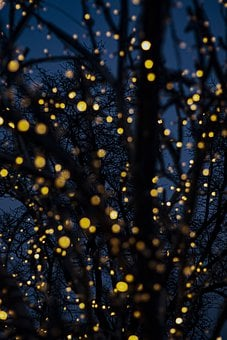
\includegraphics[width=\textwidth]{images/mult0.jpg}
        \captionof{figure}{Lichtpunkte auf dunklem Hintergrund}
        \caption*{Quelle: \cite{bib:vodafone-legt-in-pirmasens}}
        \label{fig:light-points-on-dark-bg}
    \end{subfigure}
    \hfill
    \begin{subfigure}[t]{0.3\textwidth}
        
\includegraphics[width=\textwidth]{images/mult1.png}
        \captionof{figure}{Ein Tannenbaum}
        \caption*{Quelle: \cite{bib:vodafone-legt-in-pirmasens}}
        \label{fig:tannenbaum}
    \end{subfigure}
    \hfill
    \begin{subfigure}[t]{0.3\textwidth}
        
\includegraphics[width=\textwidth]{images/mult2.jpg}
        \captionof{figure}{Eine Winterstadt}
        \caption*{Quelle: \cite{bib:vodafone-legt-in-pirmasens}}
        \label{fig:winter-city}
    \end{subfigure}


    \caption{Ein Beispiel für mehrere Bilder nebeneinander}
\end{figure}

% Example Table:
\begin{table}[!htbp] % !htbp
    \centering
    \begin{tabular}{|l|l|r|}
        \hline
        \textbf{TM Configuration}   &   \textbf{Detail-Level}   &   \textbf{Frametime}\\
        \hline
        \hline
        Tensor-800                  &   0                       &   28\\
        Tensor-800                  &   1                       &   52\\
        Tensor-800                  &   2                       &   69\\
        Tensor-800                  &   3                       &   89\\
        \hdashline
        V-Core Zenyx 33             &   0                       &   2\\
        V-Core Zenyx 33             &   1                       &   4\\
        V-Core Zenyx 33             &   2                       &   5\\
        V-Core Zenyx 33             &   3                       &   7\\
        \hdashline
        Intel iZ237-8               &   0                       &   298\\
        Intel iZ237-8               &   1                       &   448\\
        Intel iZ237-8               &   2                       &   556\\
        Intel iZ237-8               &   3                       &   767\\
        \hline
    \end{tabular}
    \caption{Eine Beispieltabelle}
    \label{tbl:renderzeiten_tm_processors}
\end{table}

% Example code:
\begin{code}
// Example code
#include <iostream>

int main(int argc, char** argv)
{
    std::cout << "Hello, World!" << std::endl;
    return 0;
}
\end{code}
